\documentclass{report}

\usepackage{graphicx}
\usepackage{float}
\usepackage{wrapfig}
\usepackage{color}
\usepackage{siunitx}
\usepackage[usenames,dvipsnames]{xcolor}
\usepackage[english]{babel}
\usepackage{amssymb}
\usepackage{geometry}

\begin{document}

\title{\textbf{Homework 5:} $\mathcal{A}x=b$: Solving systems of linear equations using Gauss-Jordan and LU decomposition}
\author{A.L. Phillips II\\
  Department of Physics, Astronomy, and Applied Physics,\\
  Rensselaer Polytechnic Institute\\
  \texttt{philla3@rpi.edu}}
 \date{26 April 2013}
 \renewcommand{\chaptername}{Assignment}
 \setcounter {chapter}{4}
\maketitle

\chapter{System of Linear Equations}

\section{Gauss-Jordan Elimination & LU Decomposition}
\begin{enumerate}

\item A system of linear equations may be written in matrix/vector notation as:
\begin{center}
$\displaystyle \mathbf{A}\vec{x}=\vec{b}$
\end{center} 
Gauss-Jordan elimination and LU decomposition are two methods which solve these types of equations. Using the Gauss-Jordan method allows  is to solve $\displaystyle \mathbf{A}\vec{x}=\vec{b}$ for $\displaystyle \vec{x}=\mathbf{A}^{-1}\vec{b}$. 
\\
\\Gauss-Jordan method then finds the inverse of $\mathbf{A}$ by multiplying the adjunct of $\mathbf{A}$ by the determinate of $\mathbf{A}$. That is, 
\begin{center}
$\displaystyle \mathbf{A}^{-1}$ = $\frac{1}{\det(\mathbf{A})}adj(\mathbf{A})$
\end{center} 

The LU decomposition method works by reducing the single matrix/vector problem into two less difficult problems. The method decomposes the original square matrix into the product of it's Upper and Lower triangular sub-matrices; thus the name LU (lower/upper). First, $\mathbf{A}$ must be manipulated to obtain both it's upper and lower triangular matrices. Then, let $\mathbf{A}=\mathbf{L}\mathbf{U}$. This implies that $\displaystyle \mathbf{L}\mathbf{U}\vec{x}=\vec{b}$ goes to $\displaystyle \mathbf{l}\vec{x}=\vec{b}$. Therefore, the problem may be decomposed into it's two component equations which are then solved and back substituted to obtain:
\begin{center}
$\displaystyle \mathbf{L}\vec{y} = \vec{b}$
\end{center} 
\begin{center}
$\displaystyle \mathbf{U}\vec{x} = \vec{y}$
\end{center} 
\end{enumerate}



\section{Resistor Arrays}
\begin{enumerate}
\item 
\begin{figure}[H]
\centering \caption{A 5 x 3 Array of Resistors(All 1$\Omega$), Voltage Source(1$v$)}
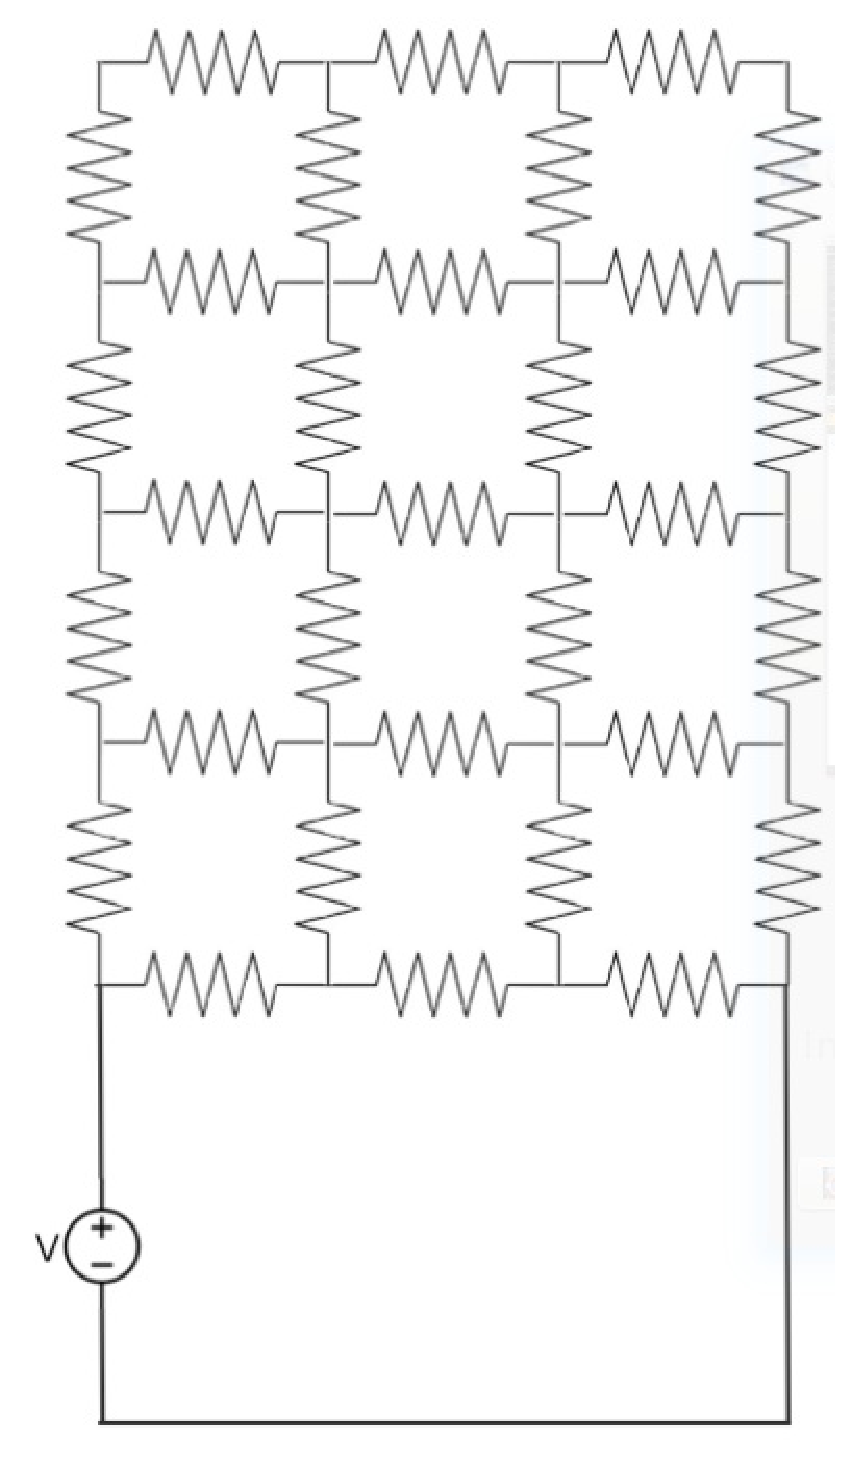
\includegraphics[scale=.42]{array.eps}
\label{sej}
\end{figure}
\\
\\In simple circuits, solving for equivalent resistance, voltage and current across series and parallel resistors is done using $\displaystyle V=iR$. To find the equivalent resistance of the entire circuit, we may find the resistance that is "felt" by the voltage source. 
\\
\\The circuits total equivalent resistance may be found by dividing the Voltage by the current through the voltage source: 
\begin{center}
$\displaystyle R_{equiv}=\frac{V}{i}$. 
\end{center}
The equivalent resistance between individual devices may be found through direct or reciprocal addition. For resistors in series, the resistances between devices increases, therefore: 
\begin{center}
$\displaystyle R_{equiv} = R_1 + R_2$ (Resistors in Series)
\end{center}
For resistors in parallel, the resistance is less then the smallest resistance of the devices in parallel, therefore:  
\begin{center}
$\displaystyle R_{equiv}=\frac{1}{R_1} + \frac{1}{R_2}$ (Resistors in Parallel)
\end{center}

In the case of a resistor array such as that depicted above, the task of solving for these concepts may range from tedious to daunting. To simplify the problem, Kirchhoff's loop rule may be implemented in order to generate a matrix/vector equation where the matrix is of resistances and the vectors are of currents and voltage. 
\\
\\
\\
\[ \left( \begin{array}{ccccccccccccc}
3&-1&0&0&0&-1&0&0&0&-1&0&0&0 \\
-1&4&-1&0&0&-1&0&0&0&0&0&0&0 \\
0&-1&4&-1&0&0&-1&0&0&0&0&0&0 \\
0&0&-1&4&-1&0&0&-1&0&0&0&0&0 \\
0&0&0&-1&4&0&0&0&-1&0&0&0&0 \\
-1&-1&0&0&0&4&-1&0&0&-1&0&0&0 \\
0&0&-1&0&0&-1&4&-1&0&0&-1&0&0 \\
0&0&0&-1&0&0&-1&4&-1&0&0&-1&0 \\
0&0&0&0&-1&0&0&-1&4&0&0&0&-1 \\
-1&0&0&0&0&-1&0&0&0&4&-1&0&0 \\
0&0&0&0&0&0&-1&0&0&-1&4&-1&0 \\
0&0&0&0&0&0&0&-1&0&0&-1&4&-1 \\
0&0&0&0&0&0&0&0&-1&0&0&-1&4 \end{array} \right)\] 
\\
\\
\\
Using standard matrix operations, the inverse of the above matrix may be found and multiplied by the voltage vector to obtain the current vector. While this task would be daunting by hand, it is a job perfectly suited for the computer. Providing both the above Resistance matrix and the Voltage Vector to the Numerical Recipes Gauss-Jordan routine returns the following vector of currents:
\\
\\
\\
\[ \left( \begin{array}{c}
0.622396 &
0.268451 &
0.121124 &
0.0541993 &
0.0208314 &
0.330286 &
0.161844 &
0.0748421 &
0.0291262 &
0.268451 &
0.121124 &
0.0541993 &
0.0208314 \end{array} \right)\] 
\\   
\\
\\
In order to solve for the equivalent resistance, me may consider Kirchhoff's junction rule which states that the current into a node is equal to the current out of that node. Applying this reasoning we may obtain the real current ($i_1$-real) around the voltage source by evaluating the nodes that the source is directly connected to. Whatever goes into one end must come out on the other. Therefore, the entry node yields the following current:
\\
\\
\begin{center}
$\displaystyle i_1$-real = ($i_1$-mesh $-$ $i_2$-mesh) $+$ $i_2$-mesh  
\end{center}
\begin{center}
$\displaystyle i_1$-real = ($0.622396 - 0.268451$) $+$ $0.268451$
\end{center}
\begin{center}
$\displaystyle i_1$-real $\approx$ $0.622396A$
\end{center}

\\Now that we know $i_1$-real, we may use $V=iR$ to solve for the equivalent resistance of the circuit. 
\begin{center}
$\displaystyle R_{equiv}=\frac{V}{i}$
\end{center}
\begin{center}
$\displaystyle R_{equiv}=\frac{1v}{0.622396A}$
\end{center}
\begin{center}
$\displaystyle R_{equiv}=\frac{1v}{0.622396A}$
\end{center}
\begin{center}
$\displaystyle R_{equiv}\approx1.60669413A$
\end{center}
\\Allowing the array of resistors to take on different dimensions yeild different equivalent resistances. The following plot depicts the equivalent resistance for arrays whose two dimensions are less than or equal to 20.

\begin{figure}[H]
\centering \caption{\textcolor{purple}{Potential} versus Resistor Array Dimensions ...}
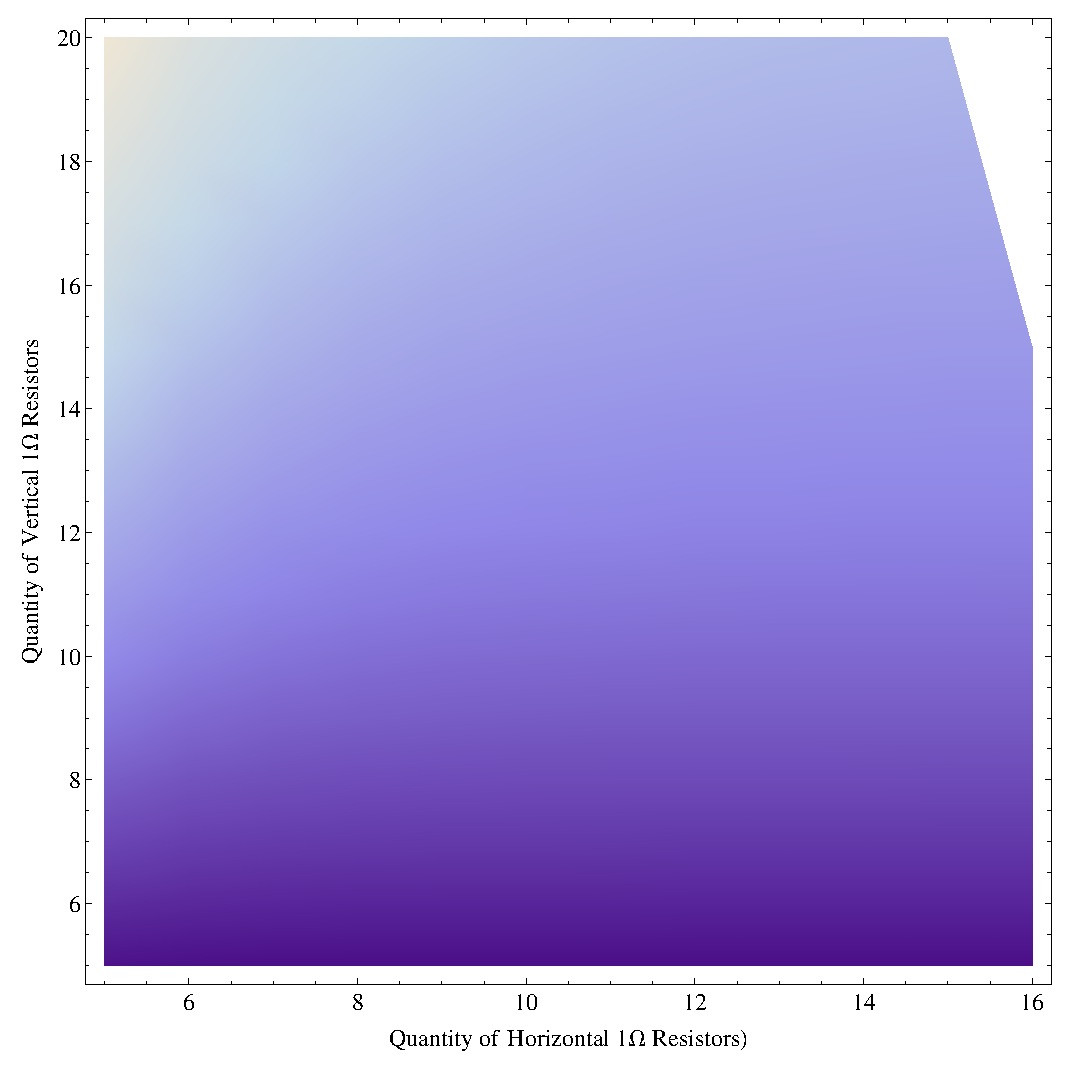
\includegraphics[scale=.72]{equivalent.eps}
\label{equiv}
\end{figure}
As may be expected, the equivalent is greatest when the quantity of horizontal resistors is maximized and the quantity of vertical resistors is minimized. That is, the more series resistors, the greater the equivalent resistance. The more parallel resistors, the less the equivalent resistance.
\\
Comparing Gauss-Jordan to LU Decomposition solutions results a significant performance gain for larger arrays. The following plot depicts the execution times required by each method to solve an $MxN$ array of resistors:
\begin{figure}[H]
\centering \caption{Execution Time of \textcolor{blue}{Gauss-Jordan} versus \textcolor{green}{LU Decomposition}}
\includegraphics[scale=.71]{time.eps}
\label{time}
\end{figure}
It may be noted from the above figure that for "larger" arrays, LU Decomposition has an approximate $\frac{2}{3}$ performance gain over Gauss-Jordan.
\\
\\The potential drop across each resistor may be found using $V=iR$. In order to voltage at each device, multiply $i$-real by resistance: 
\begin{center}
$\displaystyle V_{real} = i_{real}R$
\end{center}
\begin{center}
$\displaystyle V_{real} = i_{real}(1)$
\end{center}
\\In the case of R=1$\omega$, $V_{real} = i_{real}$, and therefore the voltage across each device may be found by finding the real current from the mesh currents as described above.
\\
\\The following plot depicts the potential drop across each resistor on a fixed $5x3$ array of resistors:
\begin{figure}[H]
\centering \caption{Potential Drop at each (2n+1)$^{th}$ Resistor in a $5x3$  Array}
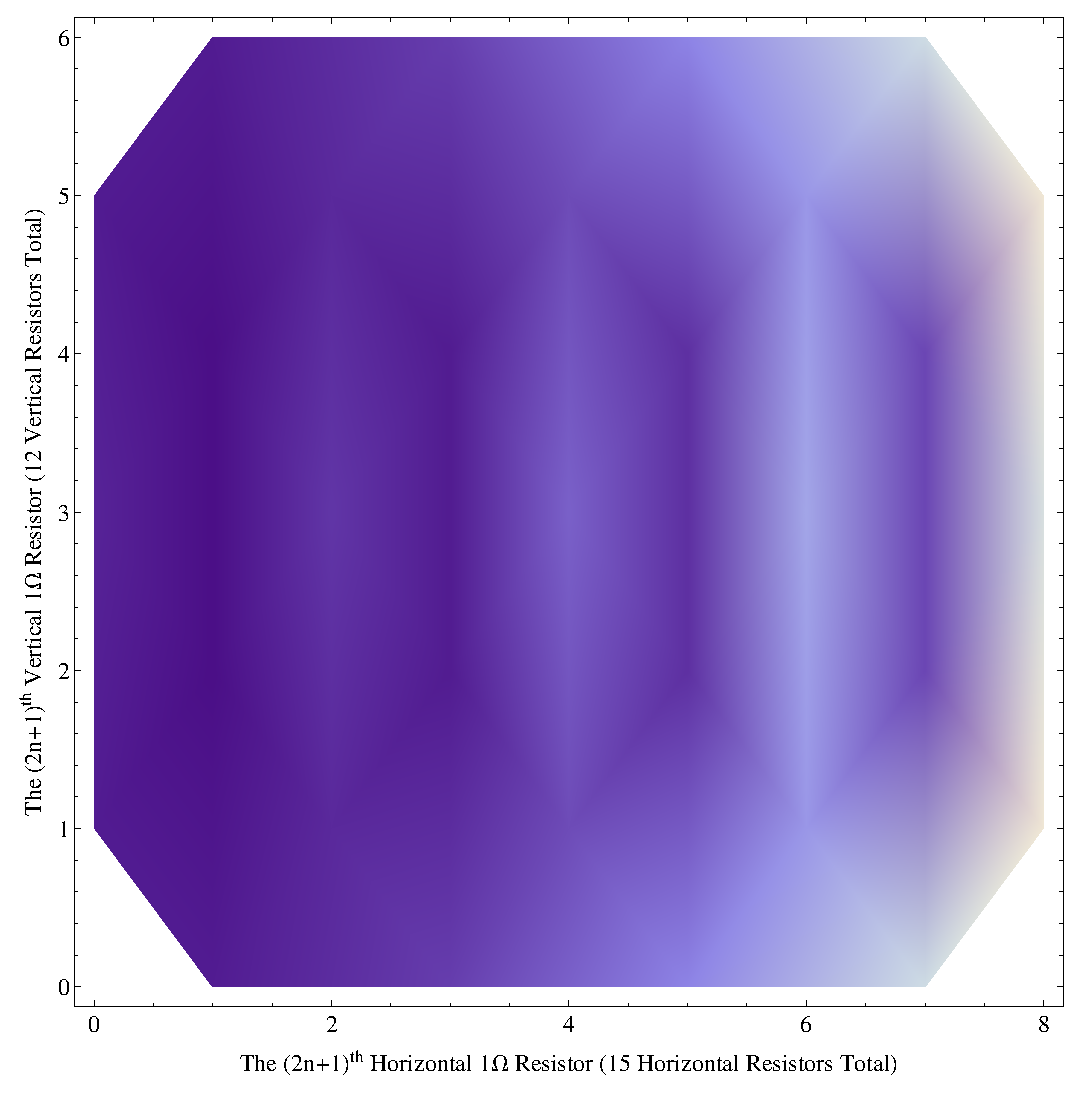
\includegraphics[scale=.81]{potdrop.eps}
\label{potdrop}
\end{figure}
*Note: As expected, the maximum voltage drops occur after the first node in the circuit and perpetuate along the left-most string of in-series resistors. 

Note also that since $V=iR$, the real current is equal to $\frac{V_{real}}{R}$. That is, $i_n$-real $=\frac{V_{real}}{R}$. We see from the above graph that voltage is a minimum at the top right of the resistor array, and therefore this is also the location of minimum current.


























\end{enumerate}
\end{document}